\documentclass{article}
\usepackage[]{graphicx}
\usepackage[]{unicode-math}
\usepackage[utf8]{inputenc}


\begin{document}


\section{Dataset}
The Aidelman dataset contains ~3.300.000 samples and each sample is labeled as an H$α$ emitting object (EM) and/or a Be star (Be). Each sample includes measurements from 10 different channels: u, g, r, H$α$, i, J, H, K, W1 and W2.


\begin{figure}
    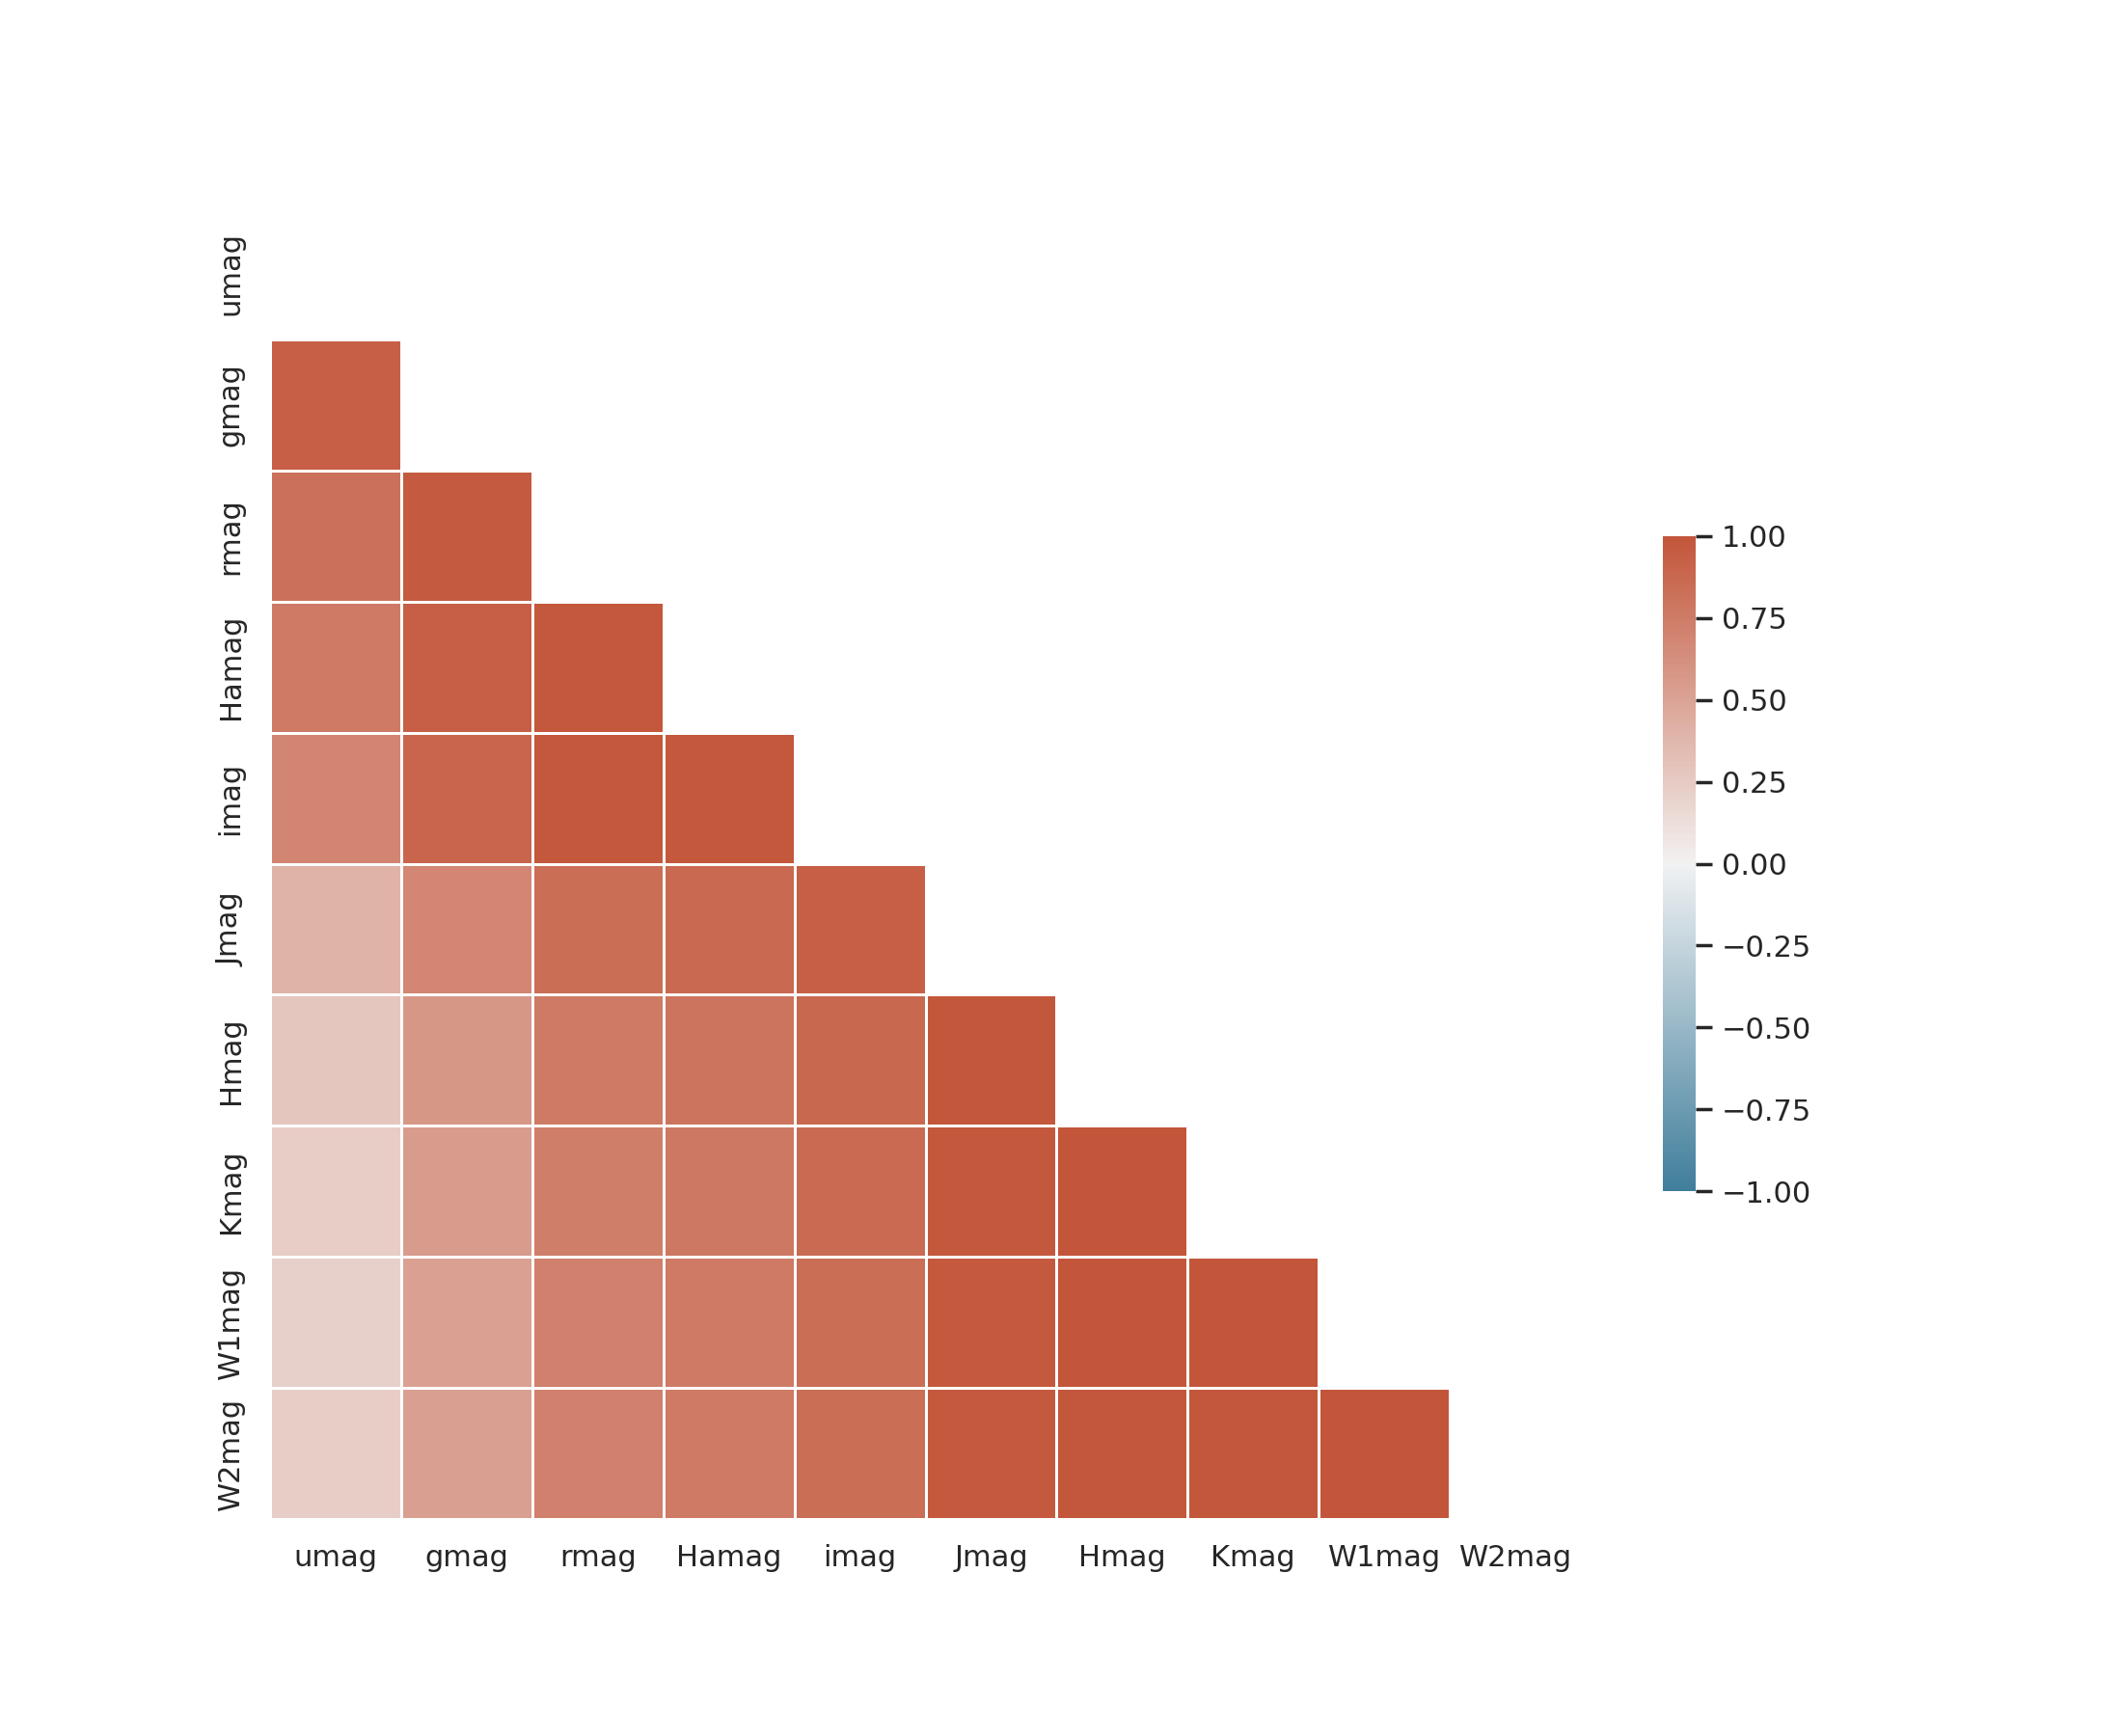
\includegraphics[width=1\linewidth]{reports/aidelman/correlation.png}
    \caption{Correlation between features}
\end{figure}

\section{Experiments}

\subsection{EM classification}
In order to establish a baseline performance for classifying EM objects, we split the dataset 80/20, obtaining training and test subsets, and we train three common models using SKLearn:

\begin{itemize}
    \item Random Forest, with a max depth of 6
    \item 3-layer neural network, with (10,10) hidden states
    \item Gradient Boosting, with 300 tree estimators
\end{itemize}

\begin{verbatim}    
    Train:                         Model    fscore  precision    recall
    0      RandomForestClassifier  0.951191   0.908095  0.998581
    1               MLPClassifier  0.954169   0.919153  0.991958
    2  GradientBoostingClassifier  0.951439   0.911145  0.995461
    Test:                         Model    fscore  precision    recall
    0      RandomForestClassifier  0.951387   0.908369  0.998682
    1               MLPClassifier  0.954212   0.919330  0.991846
    2  GradientBoostingClassifier  0.951507   0.911367  0.995345
\end{verbatim}
    
\begin{figure}
    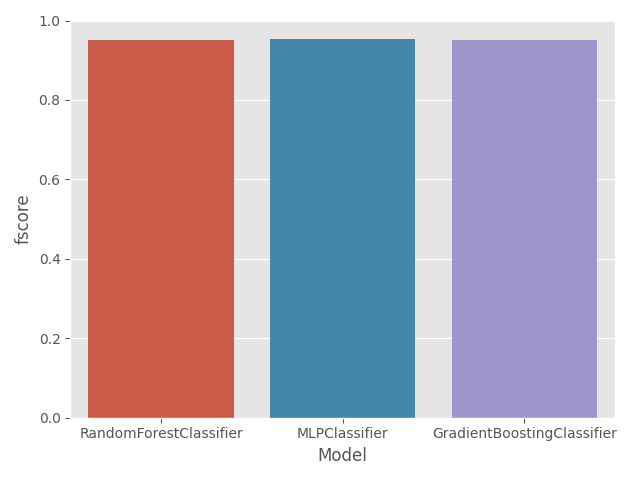
\includegraphics[width=0.49\linewidth]{plots/SKLearnClassifiers/aidelman_em_train_fscore.png}
    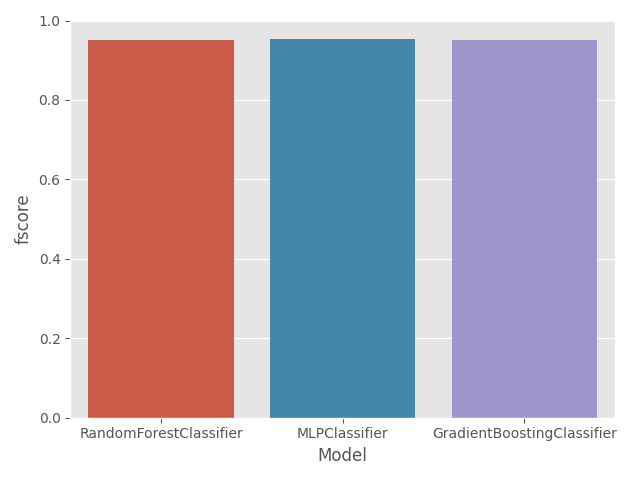
\includegraphics[width=0.49\linewidth]{plots/SKLearnClassifiers/aidelman_em_test_fscore.png}
    \caption{F-Score for train (left) and test (right) sets when classifying stars as EM or not.}
\end{figure}

\begin{figure}
    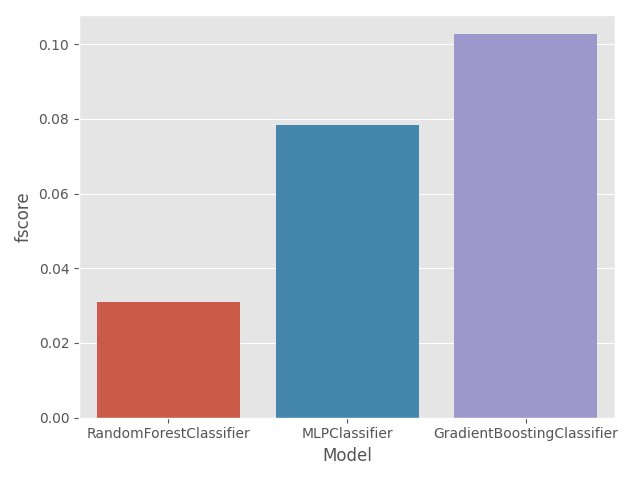
\includegraphics[width=0.49\linewidth]{plots/SKLearnClassifiers/aidelman_be_train_fscore.png}
    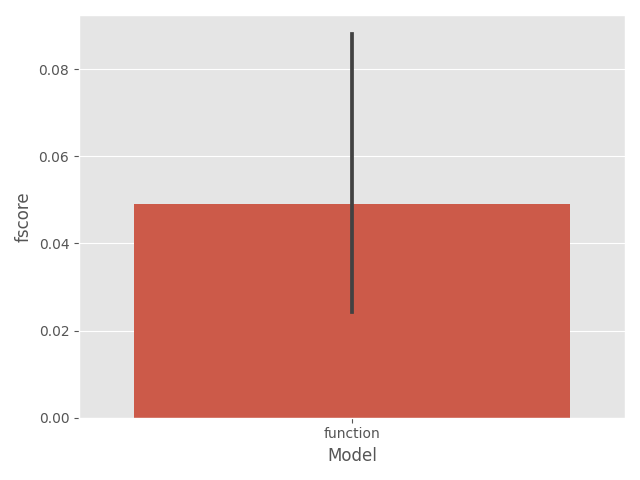
\includegraphics[width=0.49\linewidth]{plots/SKLearnClassifiers/aidelman_be_test_fscore.png}
    \caption{F-Score for train (left) and test (right) sets when classifying stars as BE or not.}
\end{figure}

\end{document}